%!TEX encoding = UTF-8 Unicode
\documentclass[12pt]{book}          %Abschlußarbeit 12pt-book
\usepackage[utf8]{inputenc}         %empfohlene Zeichenkodierung UTF-8
\usepackage[T1]{fontenc}            %empfohlene Fontkodierung
\usepackage{lmodern}                %besserer Font
\usepackage{microtype}              %bessere Zeichenabstände
\usepackage[german]{babel}          %deutsch
\usepackage{hyperref}               % um auf sections zu verweisen
\usepackage{csquotes}               % Required for fine quoting
\usepackage{enumitem}               % Required for nested arabic Enumeration
\usepackage{graphicx}               % Required for inserting images
\usepackage[Algorithmus]{algorithm} % Algorithmen
\usepackage{algpseudocode}
\usepackage{listings}
\usepackage[utf8]{inputenc}
\usepackage[T1]{fontenc}
\usepackage{listingsutf8}
\usepackage{chngcntr}
\usepackage{amsmath}

\lstset{
    literate=%
    {ä}{{\"a}}1
    {ö}{{\"o}}1
    {ü}{{\"u}}1
    {Ä}{{\"A}}1
    {Ö}{{\"O}}1
    {Ü}{{\"U}}1
    {ß}{{\ss}}1
}

\algnewcommand\algorithmicforeach{\textbf{for each}}
\algdef{S}[FOR]{ForEach}[1]{\algorithmicforeach\ #1\ \algorithmicdo}
\usepackage[
backend=biber,
style=alphabetic
]{biblatex}                         %required for citations
\usepackage[
    a4paper,
    margin=2.5cm
]{geometry}                         %Seitenmaße
\parskip.5\baselineskip

%Algorithmen
\lstdefinelanguage{JavaScript}{
  keywords={break, case, catch, continue, debugger, default, delete, do, else, finally, for, function, if, in, instanceof, new, return, switch, this, throw, try, typeof, var, void, while, with, export, interface, string, boolean, const, false, true},
  morecomment=[l]{//},
  morecomment=[s]{/*}{*/},
  morestring=[b]",
  morestring=[b]'
}
\lstset{language=JavaScript, basicstyle=\ttfamily, keywordstyle=\bfseries, showstringspaces=false}
\renewcommand{\listalgorithmname}{Algorithmenverzeichnis}
\counterwithin{algorithm}{chapter}




\addbibresource{bibliography.bib} %Imports bibliography file


%--------------TITEL-----------------
%------------------------------------
\title{
\begin{center}
   \parskip1\baselineskip

   \large
   Abschlussarbeit am LG Kooperative Systeme der FernUniversität in Hagen
   
   ~
   
   \LARGE\bfseries 
    YReduxSocket: Ein Werkzeug zur Synchronisation und Konsistenz in Webanwendungen

   \large
   Ricardo Stolzlechner
   
   9463470
   
   ricardo.stolzlechner@gmail.com
   
   Informatik Bachelor of Science
   
   Betreuerin: Dr. Lihong Ma
\end{center}
}

\author{}

\begin{document}

\maketitle

%--------------ABSTRACT-------------------
%-----------------------------------------
\chapter*{Abstract}

\newpage

%--------------VERZEICHNISSE--------------
%-----------------------------------------
\tableofcontents
%\listoftables %uncomment this if more than one table is used
\listoffigures
\listofalgorithms

\newpage

%--------------EINLEITUNG--------------
%--------------------------------------
\chapter{Einleitung}
\label{chap-einleitung}

\section{Hintergrund und Motivation}
\label{sec-hintergrund-und-motivation}

Die Webanwendung "`Yoshie.io"'\footnote{\url{https://www.yoshie.io/}} ist eine kollaborative Plattform, spezialisiert auf das Baugewerbe. Der Autor dieser Arbeit fungiert hier als technischer Leiter. Im Baugewerbe operieren die verschiedenen Gewerke häufig in isolierten Datensilos. Baupläne und ähnliche Dokumente liegen bei den Beteiligten in unterschiedlichen Versionen vor, was während der Bauphase oft zu Fehlern und damit verbundenen Mehrkosten führt. "`Yoshie.io"' bietet eine Lösung, indem es eine Plattform zur Verfügung stellt, auf der sämtliche für ein Bauvorhaben erforderlichen Dokumente zentralisiert, versioniert und zugänglich gemacht werden. 

Während der Entwicklung dieser Anwendung wurde offensichtlich, dass eine der zentralen Herausforderungen darin besteht, die Konsistenz der dargestellten Daten zu gewährleisten. Diese Anforderung lässt sich in zwei Hauptbereiche unterteilen, die unterschiedliche technologische Ansätze erfordern. Einerseits muss die Datenkonsistenz innerhalb der verschiedenen Komponenten desselben Clients sichergestellt werden. Andererseits ist es notwendig, Datenänderungen zwischen verschiedenen Clients zu synchronisieren. Basierend auf Tanenbaum und van Steen musste ein clientbasiertes Konsistenzmodell implementiert werden, welches die Eigenschaften \textit{monotones Lesen}, \textit{monotones Schreiben}, \textit{Read Your Writes} sowie eine \textit{Writes Follow Reads} Konsistenz aufweist \cite[322-325]{tanenbaum_verteilte_2008}. In diesem Zusammenhang wurden ein auf Redux basierender Datenstore und das WebSocket-Kommunikationsprotokoll als technologische Lösungen eingesetzt.

Der Aufwand für die Implementierung und Wartung der Anwendung im Bereich der Konsistenzerhaltung stieg zunehmend. Daher wurde ein Konzept entwickelt, das beide Technologien kombiniert, um so den Entwicklungsaufwand erheblich zu reduzieren. Dieses Konzept erhielt intern den Namen \textit{YReduxSocket}. Im Rahmen dieser Arbeit soll das genannte Konzept detailliert betrachtet und spezifiziert werden.

\section{Problemstellung}
\label{sec-problemstellung}

Wie bereits in Abschnitt \ref{sec-hintergrund-und-motivation} erwähnt, ergeben sich im Kontext der Konsistenzerhaltung in Webanwendungen zwei unterschiedliche Problemfelder. Diese werden in den folgenden Abschnitten näher erläutert.

\subsection{Datenkonsistenz am selben Client}
\label{subsec-datenkonsistenz-am-selben-client}

JavaScript-Frameworks wie \textit{React} oder \textit{Angular} basieren auf einer komponentenorientierten Architektur. Hierbei stellt jede Komponente ein User-Interface-Element dar, das an verschiedenen Stellen innerhalb der Anwendung eingesetzt werden kann. Diese Komponenten können weitere Unterkomponenten umfassen, wodurch ein Komponentenbaum entsteht. Typischerweise gibt es in Webanwendungen zahlreiche verschiedene Komponenten,
deren Daten im Baum ausgetauscht und synchronisiert werden müssen.

Häufig sollen verschiedene Komponenten identische Daten anzeigen. In solchen Fällen muss eine Anwendung entwickelt werden, die sicherstellt, dass die Daten zwischen diesen Komponenten synchronisiert bleiben. Aufgrund der Notwendigkeit einer losen Kopplung, bei der Unterkomponenten keine direkte Kenntnis von ihren Elternkomponenten haben, ist die Synchronisation dieser Daten keine triviale Aufgabe.

\begin{figure}[htbp]
\centering
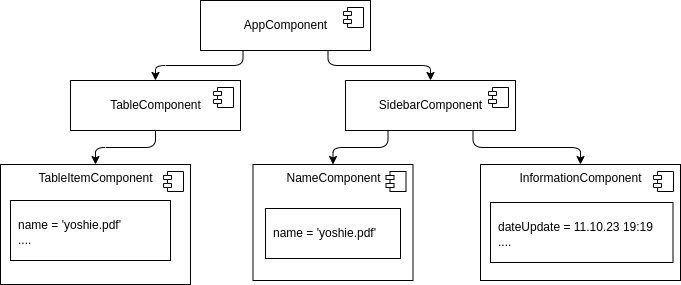
\includegraphics[height=6cm]{abbildungen/components-sync-1.png}
\caption{UML-Diagramm eines einfachen Komponentenbaums}
\label{simple-component-tree-uml}
\end{figure}

\begin{figure}[htbp]
\centering
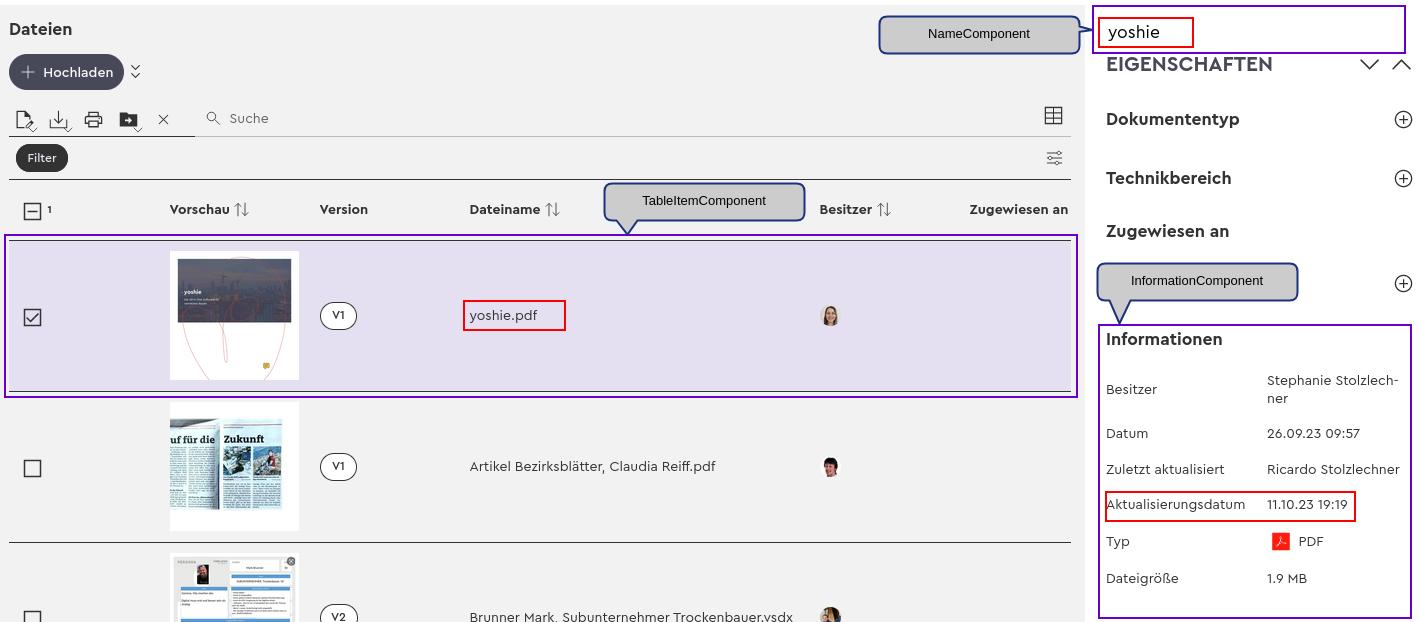
\includegraphics[height=7cm]{abbildungen/simple-comp-tree-screenshot.png}
\caption{Bildschirmausschnitt eines einfachen Komponentenbaums}
\label{simple-component-tree-screenshot}
\end{figure}

In Abbildung \ref{simple-component-tree-uml} wird ein einfacher Komponentenbaum gezeigt. Der zugehörige Bildschirmausschnitt dieses Baums ist in Abbildung \ref{simple-component-tree-screenshot} zu sehen. Die Komponenten \texttt{TableItemComponent} und \texttt{NameComponent} zeigen jeweils dasselbe Datenfeld an. Wird der Name in der \texttt{NameComponent} geändert, muss die Anwendung dafür sorgen, dass diese Information auch an die \texttt{TableItemComponent} weitergegeben wird. Zudem muss das Aktualisierungsdatum in der \texttt{InformationComponent} aktualisiert werden.

Verschiedene Ansätze, um die notwendige Synchronisierung zu erreichen, werden in späteren Kapiteln detailliert betrachtet und miteinander verglichen.

\subsection{Datenkonsistenz zwischen verschiedenen Clients}
\label{subsec-datenkonsistenz-zwischen-zwei-verschiedenen-clients}

In einer Webanwendung arbeiten verschiedene Clients oft mit denselben Daten. Wenn beispielsweise zwei Benutzerinnen gleichzeitig dieselbe Ansicht, wie in Abbildung \ref{simple-component-tree-screenshot} dargestellt, geladen haben, und eine von ihnen den Namen über die \texttt{NameComponent} ändert, muss gewährleistet sein, dass diese Änderung auch bei der anderen Benutzerin sichtbar wird. Daher ist es erforderlich, einen Mechanismus zu etablieren, der bei Datenänderungen alle betroffenen Teilnehmer synchron hält. Verschiedene Ansätze zur Lösung dieses Problems werden in späteren Abschnitten vorgestellt.


\section{Ziele der Arbeit}
\label{sec-ziele-der-arbeit}

Wie bereits erwähnt, existieren diverse Ansätze zur Lösung der beiden beschriebenen Probleme. Das Konzept \textit{YReduxSocket} zielt darauf ab, beide Konsistenzanforderungen zu vereinheitlichen und gemeinsam zu adressieren. Hierbei wird auf jedem Client ein eigner auf Redux basierender Datenstore verwendet. Diese Datenstores werden anschließend mithilfe des WebSocket-Kommunikationsprotokolls, welches von einer zentralen Serverinstanz gesteuert wird, synchronisiert. Ein besonderer Fokus bei der Entwicklung von \textit{YReduxSocket} lag auf der Entwicklerfreundlichkeit. Das Konzept minimiert die bei Funktionserweiterungen notwendigen Änderungen bezüglich des Konsistenzverhaltens. Dies trägt zur Reduzierung von Entwicklungsfehlern bei und verbessert somit das Konsistenzverhalten von Webanwendungen.

Das primäre Ziel dieser Arbeit besteht darin, \textit{YReduxSocket} und die zugrundeliegenden Technologien generisch zu spezifizieren. Ein besonderes Augenmerk liegt auf der detaillierten Untersuchung des Konsistenzverhaltens des Konzepts. Zusätzlich wird die vorgestellte Spezifikation implementiert, um deren praktische Anwendbarkeit zu testen. \\

\section{Struktur der Arbeit}
\label{sec-struktur-der-arbeit}

Zu Beginn werden in Kapitel \ref{chap-grundlagen} die grundlegenden Konzepte erörtert, die für das Verständnis der weiteren Arbeit essenziell sind. Dabei liegt der Fokus auf Single Page Applications, der komponentenbasierten Webentwicklung, dem zentralen Redux-basierten Datenstore sowie dem WebSocket-Kommunikationsprotokoll. Ferner wird definiert, welche Voraussetzungen für den Einsatz von \textit{YReduxSocket} erfüllt sein müssen. Im abschließenden Teil dieses Kapitels wird ein Ansatz vorgestellt, wie ein Datenstore mittels WebSocket-Nachrichten synchronisiert werden kann.

Das anschließende Kapitel \ref{chap-y-redux-socket} ist dem Konzept \textit{YReduxSocket} gewidmet. Hier wird das Konzept zunächst generisch vorgestellt und spezifiziert. Der Abschnitt \ref{sec-konsistenzverhalten} vertieft das Thema, indem das Konsistenzverhalten von \textit{YReduxSocket} genauer beleuchtet wird. Das Kapitel schließt mit einem Vergleich von \textit{YReduxSocket} mit dem in Abschnitt \ref{sec-datenstore-mit-websocket-herkoemmlicher-ansatz} vorgestelltem Ansatz.

In Kapitel \ref{chap-implementierung-und-tests} wird vorgestellt, wie \textit{YReduxSocket} implementiert werden kann. Abschnitt \ref{sec-impl-architektur} geht zunächst auf die gewählte Software-Architektur ein. Der Abschnitt \ref{sec-impl-angular} behandelt die clientseitige Implementierung, welche dem Framework Angular zugrunde liegt. Abschließend behandelt der Abschnitt \ref{sec-impl-asp-net} die Implementierung der Serverseite im Frameworek ASP.Net.

Die Arbeit wird mit Kapitel \ref{chap-fazit} abgerundet. In diesem Abschnitt werden die erzielten Ergebnisse zusammengefasst, die Lösung validiert und potenzielle Verbesserungen des Konzepts aufgezeigt. 



%--------------GRUNDLAGEN--------------
%--------------------------------------
\chapter{Grundlagen}
\label{chap-grundlagen}

In diesem Kapitel werden grundlegende Konzepte vorgestellt, die eine solide Basis für das Verständnis des weiteren Inhalts dieser Arbeit bilden. Es werden außerdem jene Voraussetzungen definiert, die für den erfolgreichen Einsatz von \textit{YReduxSocket} notwendig sind.

\section{Single Page Applications (SPAs)}
\label{sec-single-page-applications}

Single Page Applications (SPAs) zeichnen sich dadurch aus, dass die gesamte Anwendung im Webbrowser des Benutzers ausgeführt wird. Eine SPA wird von einem Webserver bereitgestellt, der eine \texttt{index.html}-Datei enthält. Diese wird ausgeliefert, sobald die entsprechende URL im Webbrowser aufgerufen wird. In der \texttt{index.html} befindet sich ein \texttt{script}-Tag, das auf den erforderlichen JavaScript-Code für die Ausführung der Anwendung verweist. Dieser Code wird vom Browser heruntergeladen und ausgeführt. Nach dem initialen Ladevorgang beschränkt sich die Rolle des Webservers darauf, statische Ressourcen wie Schriftarten oder Bilder nachzuladen. Die benötigten HTML-Elemente für die Darstellung werden ausschließlich über JavaScript generiert und aktualisiert. Für die Entwicklung von SPAs werden verschiedene etablierte Frameworks wie \textit{Angular}, \textit{React} und \textit{Vue} verwendet, die die DOM-API des Webbrowsers abstrahieren und somit die Entwicklung vereinfachen. Dies steht im Gegensatz zu klassischen Webanwendungen, bei denen der HTML-Code serverseitig generiert und ausgeliefert wird, bekannt als serverseitiges Rendering \cite[1]{hartmann_react_2020}.

\section{Client-Kommunikation}
\label{sec-sync-async-comm}

In Abbildung \ref{spa-lonely-architecture} ist die Prozessarchitektur von Single Page Applications graphisch dargestellt. Dabei ist ersichtlich, dass es für die Clients ohne Erweiterung keine Möglichkeit gibt, untereinander zu kommunizieren.

\begin{figure}[htbp]
\centering
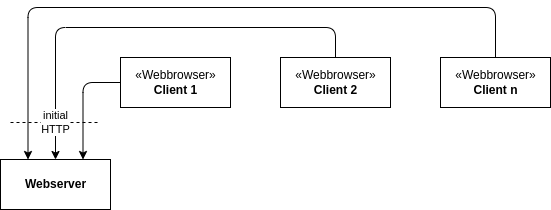
\includegraphics[height=4cm]{abbildungen/spa/spa-lonely.png}
\caption{Prozessarchitektur von Single Page Applications}
\label{spa-lonely-architecture}
\end{figure}

Die Clients können nun auf zwei verschiedene Arten kommunizieren: synchron oder asynchron. Unter synchroner Kommunikation versteht man dabei eine Form der Kommunikation, bei der der Austausch für den Sender und den Empfänger gleichzeitig abläuft. Bei der asynchronen Kommunikation kann das Empfangen durchaus zu einem anderen Zeitpunkt als das Senden passieren \cite[1]{cacciagrano_synchronous_2001}. Ein prominentes Beispiel für eine synchrone Kommunikation ist ein Telefongespräch, hingegen ist das Versenden einer E-Mail ein asynchroner Kommunikationsvorgang.

In den folgenden Abschnitten wird beleuchtet, welche Architekturerweiterungen an einer SPA getroffen werden müssen, um zunächst synchrone Kommunikation, dann asynchrone Kommunikation und abschließend beide Arten zu ermöglichen.

\subsection{asynchrone Kommunikation}
\label{subsc-async-comm}

Um asynchrone Kommunikation zwischen den Clients einer Single-Page-Anwendung (SPA) zu realisieren, ist eine zentrale Datenbasis erforderlich. Diese lässt sich effektiv mittels einer Datenbank umsetzen. Um Interaktionen mit der Datenbank – wie das Abrufen, Hinzufügen oder Modifizieren von Daten – zu erleichtern, empfiehlt es sich, einen Server als Vermittler zwischen den Clients und der Datenbank einzusetzen. Dieser Server kann eine HTTP-API (Application Programming Interface) bereitstellen, die spezifische Funktionen für Datenbankoperationen über HTTP-Methoden anbietet. Darüber hinaus kann der Server genutzt werden, um verschiedene Sicherheitsmaßnahmen zu implementieren. Ein Beispiel hierfür ist die Authentifizierung der Clients, die notwendig sein kann, bevor sie Datenbankabfragen starten dürfen. Abbildung \ref{spa-async-comm-architecture} illustriert die Erweiterung der SPA-Architektur, um asynchrone Kommunikation über einen gemeinsamen Speicher zu ermöglichen.

\begin{figure}[htbp]
\centering
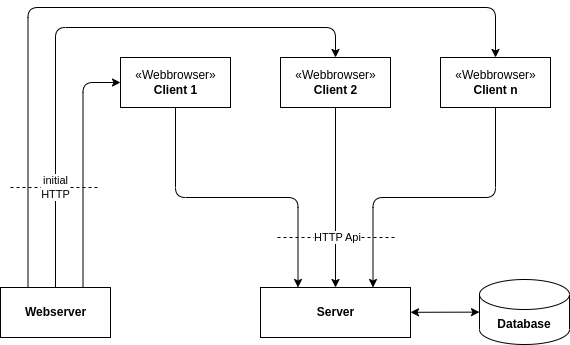
\includegraphics[height=7cm]{abbildungen/spa/spa-async-comm.png}
\caption{Prozessarchitektur von SPA's mit asynchroner Kommunikation} 
\label{spa-async-comm-architecture}
\end{figure}

Ein wesentlicher Nachteil dieser Kommunikationsmethode ist die Unfähigkeit, Echtzeit-Aktualisierungen zu unterstützen. Angenommen, sowohl Client 1 als auch Client 2 haben dieselben Daten geladen, und Client 1 beschließt, diese Daten zu ändern. Aufgrund der Beschaffenheit des HTTP-Protokolls, welches zustandslos ist und keine dauerhafte Verbindung zu seinen Clients unterhält, kann der Server Client 2 nicht proaktiv über die Änderungen informieren. Der Server reagiert lediglich auf eingehende HTTP-Anfragen mit entsprechenden Antworten. Infolgedessen verbleiben die Daten auf Client 2 so lange veraltet, bis dieser erneut eine Anfrage an den Server stellt, um die von Client 1 modifizierten Daten abzurufen.

\subsection{synchrone Kommunikation}
\label{subsc-sync-comm}

Um den Clients einer Anwendung die Möglichkeit zur synchronen Kommunikation zu bieten, können Technologien wie Long Polling oder WebSockets zum Einsatz kommen \cite[182]{ackermann_webentwicklung_2021}. In diesem Kontext konzentriert sich die Diskussion auf das WebSocket-Protokoll, welches auf der Basis von TCP bidirektionale Verbindungen zwischen Clients und Server ermöglicht, da \textit{YReduxSocket} spezifisch eine WebSocket-Verbindung voraussetzt.


\begin{figure}[htbp]
\centering
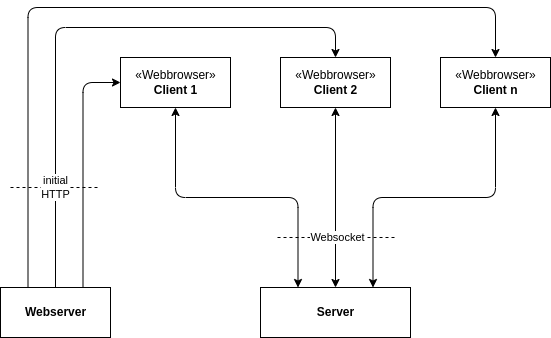
\includegraphics[height=7cm]{abbildungen/spa/spa-sync-comm.png}
\caption{Prozessarchitektur von SPA's mit synchroner Kommunikation} 
\label{spa-sync-comm-architecture}
\end{figure}

Bei einer WebSocket-Verbindung muss der Client den Verbindungsaufbau initiieren. Ist die Verbindung einmal etabliert, kann jedoch auch der Server aktiv Daten an den Client übermitteln \cite[184-185]{ackermann_webentwicklung_2021}. Um eine Überflutung mit irrelevanten Daten zu vermeiden, kann es notwendig sein, dass Clients sich für bestimmte Updates registrieren, anstatt dass der Server bei jeder neuen Nachricht einen Broadcast an alle verbundenen Clients sendet. Abbildung \ref{spa-sync-comm-architecture} illustriert die Erweiterung der SPA-Prozessarchitektur um synchrone Kommunikation mittels WebSocket zu ermöglichen. So kann beispielsweise eine Nachricht von Client 1 über den Server an Client 2 weitergeleitet werden.

Ein Nachteil der rein synchronen Kommunikation ist, dass alle Clients permanent mit dem Server verbunden sein müssen. Ein Client, der sich zu einem späteren Zeitpunkt verbindet, kann keine Nachrichten empfangen die vor seiner Verbindung gesendet wurden. Um dieses Problem zu lösen und somit den Zugriff auf frühere Nachrichten zu ermöglichen, ist der Einsatz eines Datenspeichers erforderlich.

\subsection{synchrone und asynchrone Kommunikation}
\label{subsc-sync-and-async-comm}

Wie bereits in den Abschnitten \ref{subsc-async-comm} und \ref{subsc-sync-comm} diskutiert, bringt jede Kommunikationsform – die synchrone als auch die asynchrone – spezifische Nachteile mit sich. Die Kombination beider Ansätze ermöglicht es jedoch, diese Einschränkungen zu überwinden, indem die Stärken der jeweils anderen Technologie genutzt werden. Durch die Verwendung einer Datenbank als zentralen Speicher können Änderungen in Echtzeit über das WebSocket-Protokoll an alle verbundenen Clients kommuniziert werden.

Für die Implementierung einer Single Page Application (SPA), die sowohl synchrone als auch asynchrone Kommunikation unterstützt, wie es \textit{YReduxSocket} voraussetzt, ist eine dedizierte Serverinstanz erforderlich. Diese Instanz stellt eine HTTP-API bereit und ermöglicht gleichzeitig die Einrichtung einer WebSocket-Verbindung. Zudem verwaltet und speichert sie die Anwendungsdaten in einer Datenbank. Alle Kommunikationsprozesse zwischen den Clients werden über diese Serverinstanz abgewickelt, die als eigenständiger Prozess fungiert und nicht mit dem Webserver, der die SPA ausliefert, verwechselt werden sollte. Im weiteren Verlauf wird der Begriff "`Server"' speziell für diese separate Serverinstanz verwendet. Abbildung \ref{spa-sync-and-async-comm-architecture} zeigt die für \textit{YReduxSocket} erforderliche Prozessarchitektur, wobei jedes Rechteck im Diagramm einen unabhängigen Prozess symbolisiert.

\begin{figure}[htbp]
\centering
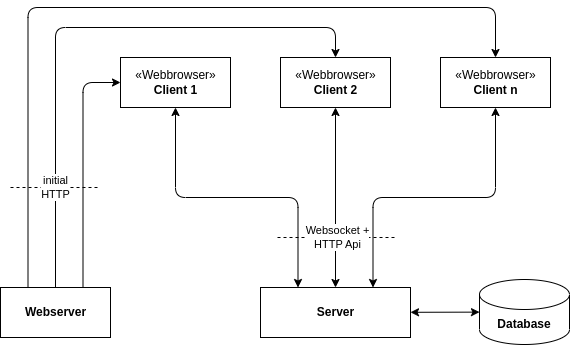
\includegraphics[height=7cm]{abbildungen/spa/spa-sync-and-async-comm.png}
\caption{Von \textit{YReduxSocket} vorausgesetzte Prozessarchitektur} 
\label{spa-sync-and-async-comm-architecture}
\end{figure}

Es ist zudem wichtig zu betonen, dass \textit{YReduxSocket} die Nutzung genau einer Datenbank vorsieht, die als verlässliche Quelle der Wahrheit (Single Source of Truth) dient.

\section{Transaktionen und ACID-Eigenschaften}
\label{sec-acid-prinzipien}

Wie in Abbildung \ref{spa-sync-and-async-comm-architecture} dargestellt, greifen mehrere Clients gleichzeitig auf den Server zu. In solchen Szenarien kann es vorkommen, dass Clients gleichzeitig dieselben Daten in der Datenbank manipulieren wollen. Um parallele Serverzugriffe zu ermöglichen, setzt \textit{YReduxSocket} den Einsatz einer Datenbank voraus, die Transaktionen unterstützt, welche den ACID-Eigenschaften entsprechen. Dies trifft beispielsweise auf gängige relationale Datenbanken zu.

\begin{algorithm}
\caption{Transaktion in einer relationalen Datenbank}
\label{alg-transaction-relational-database}
\begin{lstlisting}
transaction = createTransaction();
transaction.start();
try {
    act(); // Führt Datenbankänderungen durch
    transaction.commit();
} catch {
    transaction.rollback();
}
\end{lstlisting}
\end{algorithm}

Algorithmus \ref{alg-transaction-relational-database} illustriert das Transaktionsprinzip in einem an JavaScript angelehnten Pseudocode. Zunächst wird eine Transaktion erzeugt und gestartet. Anschließend wird versucht, Datenbankänderungen mit der Methode \texttt{act()} durchzuführen. Bei Erfolg wird die Transaktion mit \texttt{transaction.commit()} bestätigt. Vor dieser Bestätigung haben die Änderungen keine nach außen sichtbaren Auswirkungen. Schlägt der Versuch jedoch fehl, werden alle in \texttt{act()} vorgenommenen Änderungen durch \texttt{transaction.rollback()} rückgängig gemacht.

Nach Tanenbaum und van Steen muss eine Transaktion folgende Schlüsseleigenschaften aufweisen \cite[38, 39]{tanenbaum_verteilte_2008}: 
\begin{enumerate}
    \item \textbf{Atomic}: Die Transaktion definiert eine atomare Operation, d.h., sie wird entweder vollständig oder gar nicht ausgeführt.
    \item \textbf{Consistent}: Die Transaktion muss konsistent sein. Nach ihrem Abschluss müssen alle Invarianten, die an die Daten gestellt werden, erfüllt sein. Wurde beispielsweise ein Datensatz während der Transaktion verändert, muss ein eventuell vorhandenes Aktualisierungsdatum entsprechend gesetzt sein.
    \item \textbf{Isolated}: Transaktionen müssen isoliert oder serialisierbar sein. Dies bedeutet, dass sich parallel ablaufende Transaktionen nicht gegenseitig beeinflussen dürfen.
    \item \textbf{Durable}: Diese Eigenschaft beschreibt die Dauerhaftigkeit einer Transaktion. Sie gewährleistet, dass die Ergebnisse der Transaktion auch nachfolgende Systemfehler überstehen.
\end{enumerate}


\section{Komponentenbasierte Webentwicklung}
\label{sec-komponentenbasierte-webentwicklung}

Wie im Abschnitt \ref{sec-single-page-applications} erwähnt, erleichtern Frameworks den Aufbau von Single Page Applications (SPAs), indem sie auf einer komponentenbasierten Architektur aufbauen. Eine Komponente gliedert sich grundsätzlich in zwei Teile: Der erste Teil, in einer Art HTML definiert, beschreibt die Darstellung der Komponente im Browser. Der zweite Teil, mit JavaScript oder TypeScript (einer typisierten Variante von JavaScript) formuliert, definiert die logische Funktionalität der Komponente, einschließlich Methoden für Nutzerinteraktionen.

Jede Komponente kann im HTML-Teil weitere Unterkomponenten beinhalten, wodurch ein Komponentenbaum gebildet wird. Die Komponenten stehen so in einer Eltern-Kind-Beziehung zueinander.

In Webanwendungen müssen viele Komponenten miteinander kommunizieren. Dafür stellen Frameworks verschiedene Datenbindungsmechanismen zur Verfügung. Eine Eltern-Komponente kann Daten über einen Eingabeparameter an eine Kind-Komponente übergeben. Kind-Komponenten können Ausgabeparameter bereitstellen, über die sie die Eltern-Komponenten bezüglich Datenänderungen informieren. Wenn Kind-Komponenten diese Ausgabeparameter aktualisieren, wird die Eltern-Komponente automatisch benachrichtigt, sofern sie sich auf diese registriert hat.

\begin{figure}[htbp]
\centering
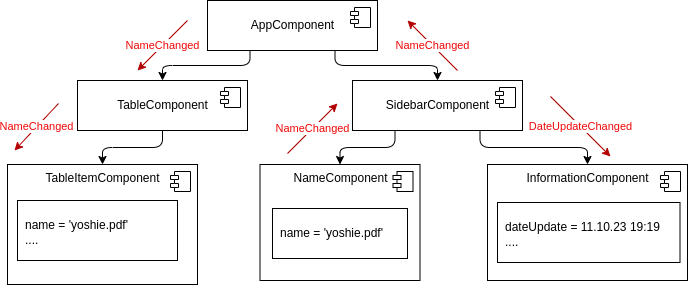
\includegraphics[height=6.5cm]{abbildungen/components-sync-data-binding.png}
\caption{Datenbindungsmechanismen: Datenfluss im Komponentenbaum}
\label{components-sync-data-binding}
\end{figure}

Abbildung \ref{components-sync-data-binding} demonstriert den Datenfluss im Komponentenbaum bei Nutzung der Datenbindungsmechanismen. Ändert sich beispielsweise der Name in der \texttt{NameComponent}, löst diese Komponente einen Ausgabeparameter aus, für den sich die übergeordnete \texttt{SidebarComponent} registriert hat. Diese informiert dann die \texttt{AppComponent} und aktualisiert einen Eingabeparameter für die \texttt{InformationComponent}, um das geänderte Aktualisierungsdatum zu melden. Die Hauptkomponente aktualisiert daraufhin ihren Eingabeparameter für die \texttt{TableComponent}, die wiederum eine \texttt{TableItemComponent} benachrichtigt. Letztgenannte kann dann ihren angezeigten Wert aktualisieren.

Bei größeren Komponentenbäumen oder wenn mehrere Komponenten denselben Datensatz anzeigen sollen, stößt dieser Ansatz jedoch an seine Grenzen. Hier bietet sich die Verwendung von Services an. Ein Service ist eine global verfügbare JavaScript-Klasse, die einmalig im Programm initialisiert wird. Die verschiedenen Frameworks bieten Mechanismen, um solche Services zu erstellen und global verfügbar zu machen.


\begin{figure}[htbp]
\centering
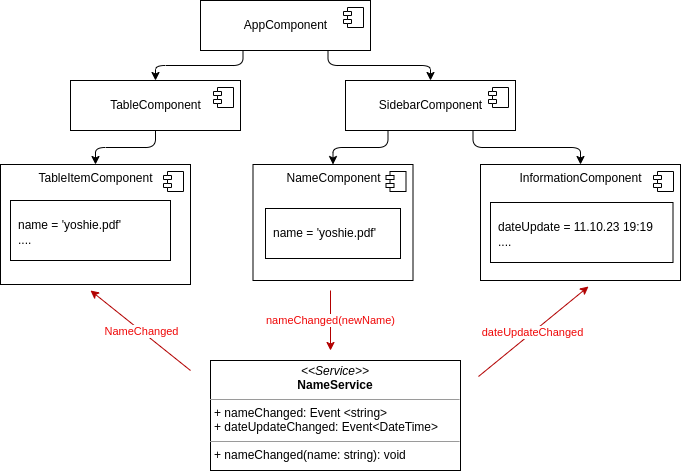
\includegraphics[height=9.5cm]{abbildungen/components-sync-service.png}
\caption{globaler Service: Datenfluss im Komponentenbaum}
\label{components-sync-service}
\end{figure}

Im Beispiel in Abbildung \ref{components-sync-service} wird ein \texttt{NameService} genutzt. Dieser Service bietet eine Methode \texttt{nameChanged}, die von der \texttt{NameComponent} bei Änderungen aufgerufen wird. Die Methode löst dann die Events \texttt{nameChanged} und \texttt{dateUpdateChanged} aus. Haben sich die \texttt{TableItemComponent} und die \texttt{InformationComponent} auf diese Events registriert, werden sie entsprechend benachrichtigt und können ihre angezeigten Werte aktualisieren.

Bei der Entwicklung mit Services bleibt jedoch das Problem der doppelten Datenhaltung bestehen. Im besprochenen Beispiel existiert die Zeichenkette \texttt{name} sowohl in der \texttt{TableItemComponent} als auch in der \texttt{NameComponent}. Dieses Problem lässt sich durch die Verwendung eines zentralen Datenstores auf Basis von Redux umgehen. Dieses Konzept wird im nächsten Abschnitt näher erläutert.


\section{Zentraler Redux-basierter Datenstore}
\label{sec-zentraler-redux-datenstore}

Mit zunehmender Anzahl von Komponenten in einer Anwendung wächst auch die Komplexität des zugrundeliegenden Codes, hauptsächlich durch die Notwendigkeit, Daten zwischen den Komponenten zu synchronisieren und einen konsistenten Zustand zu gewährleisten. Um diese Komplexität zu verringern, empfiehlt sich die Verwendung eines zentralen Stores, der auf Redux basiert (siehe Abschnitt \ref{sec-komponentenbasierte-webentwicklung}). Dieser Store wird auf der Clientseite implementiert und fungiert als eigenständige Softwareschicht, die zwischen dem User-Interface (den Komponenten) und der Serveranbindung vermittelt. Jeder Client verfügt somit über einen eigenen, individuellen Store.

\begin{figure}[htbp]
\centering
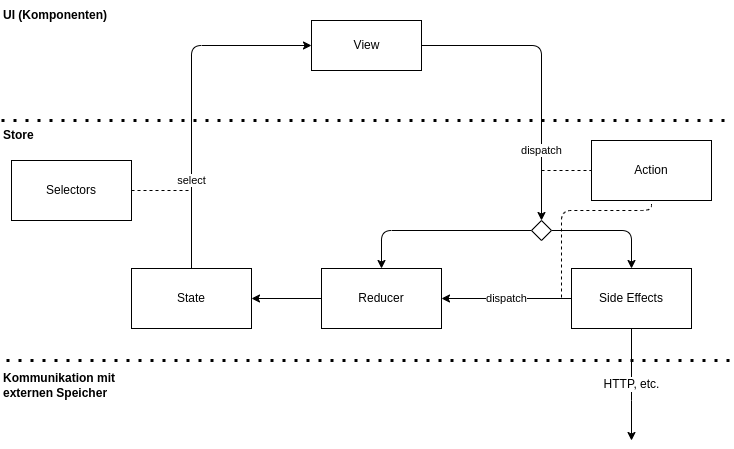
\includegraphics[height=9cm]{abbildungen/redux-interfaces.png}
\caption{Redux-basierter Store: Schnittstellen}
\label{abb-redux-interfaces}
\end{figure}

Redux, entwickelt von Dan Abramov, ist eine Implementierung des von Facebook definierten Designpatterns Flux. Dieses Pattern sieht einen unidirektionalen Datenfluss vor, wie in Abbildung \ref{abb-redux-interfaces} dargestellt. Der Store verwaltet den gesamten Anwendungszustand bezüglich der darzustellenden Daten. Er bietet Vorteile gegenüber den im vorherigen Abschnitt beschriebenen Konzepten, indem er Datenstrukturen und die gesamte Logik zur Zustandsaktualisierung an einer definierten Stelle konzentriert – bekannt als Single Source of Truth. Zusätzlich verbessert ein zentraler Store nicht nur die Performance, sondern erleichtert auch die Testbarkeit \cite[31-32]{farhi_adding_2017}.

Für eine detaillierte Beschreibung eines Redux-basierten Stores wird auf das bereits verwendete Beispiel zurückgegriffen (siehe auch Abschnitt \ref{sec-komponentenbasierte-webentwicklung}). Dabei wird die Implementierung NgRx \footnote{\url{https://ngrx.io/}}, welche im Framework Angular eingesetzt werden kann, verwendet.

\begin{figure}[htbp]
\centering
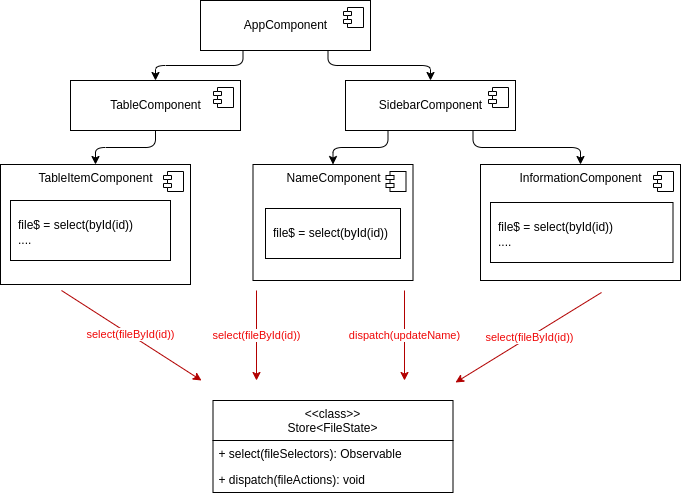
\includegraphics[height=11cm]{abbildungen/easy-state.png}
\caption{Redux-basierter Store: Datenfluss im Komponentenbaum}
\label{redux-easy-state}
\end{figure}

In Abbildung \ref{redux-easy-state} wird illustriert, wie die Komponenten mit dem Store interagieren können, um Daten abzurufen oder Datenänderungen zu veranlassen. Im Folgenden wird zunächst detailliert auf die Schnittstellen eines Stores eingegangen. Anschließend werden die Kernkonzepte eines auf Redux basierenden Stores – darunter der State, die Selektoren, die Actions, der Reducer sowie die Side Effects – ausführlich erläutert.

\subsection{Schnittstellen}
\label{subsec-store-interfaces}

 Der Store, der wie ein Service global zugänglich ist, bietet als Schnittstelle zum User Interface (den Komponenten), zwei Methoden an: Mit der Methode \texttt{select}, der ein \texttt{Selektor} übergeben wird, kann ein Ausschnitt des States abgeholt werden. Die Methode gibt kein festes Ergebnis, sondern ein \texttt{Observable} zurück, eine Art Stream. Die Komponente kann sich bei diesem \texttt{Observable} anmelden und wird bei jeder Datenänderung informiert. Um eine Datenänderung zu veranlassen, wird die Methode \texttt{dispatch} verwendet. Dieser wird eine \texttt{Action} übergeben, die definiert, wie die Änderung aussehen soll. Die \texttt{dispatch} Methode gibt keinen Wert zurück, betrifft die gewünschte Änderung jedoch einen Teil des Stores, auf den sich eine Komponente vorab über den Selektor angemeldet hat, wird im gelieferten \texttt{Observable} automatisch ein neuer Wert emittiert.

 Als weitere Schnittstelle bietet der Store die Möglichkeit, über sogenannte Side Effects mit externen Systemen zu kommunizieren, beispielsweise um Anfragen an externe Speicherlösungen zu senden, die etwa durch einen Server implementiert sein könnten. Eine detaillierte Erörterung der Side Effects erfolgt im Abschnitt \ref{subsec-side-effects}.

\subsection{State}
\label{subsec-state}


Der State wird in Form eines einfachen JavaScript-Objekts implementiert. Dieses Objekt wird dazu verwendet den gesamten Zustand der Anwendung abzubilden. Zu Beginn der Anwendung mit vorgegebenen Startwerten initialisiert. Es ist wichtig zu betonen, dass der State ausschließlich lesbar ist; Änderungen am State sind ausschließlich über definierte Reducer-Funktionen möglich, die mittels der \texttt{dispatch}-Funktion aufgerufen werden. Für die Definition des JavaScript-Objekts wird in NgRx ein Interface erstellt, in dem alle benötigten Felder definiert sind. Weiterhin muss eine Konstante definiert werden, die dem Interface entspricht und den initialen Zustand des State festlegt.

\begin{algorithm}
\caption{Statedefinition in NgRx}
\label{alg-stadedefinition-in-ng-rx}
\begin{lstlisting}
export interface FileState {
   entities: {[id: string]: FileObject};
   loaded: boolean;
   loading: boolean;
}

export const initialFileState : FileState = {
    entities: {},
    loaded: false,
    loading: false
}
\end{lstlisting}
\end{algorithm}

Algorithmus \ref{alg-stadedefinition-in-ng-rx} zeigt die Statedefinition für das Beispiel, wie in Abbildung \ref{redux-easy-state} dargestellt. Die beiden Flags \texttt{loaded} und \texttt{loading} geben an, ob die Daten bereits geladen wurden bzw. ob der Ladevorgang bereits gestartet wurde. Die tatsächlichen Daten sind in einem JavaScript-Objekt in Form eines Dictionaries oder einer HashMap abgelegt, wobei die \texttt{id} des \texttt{FileObject} dem Schlüssel und das \texttt{FileObject} selbst dem Wert entspricht. Der Vorteil dieses Ansatzes ist, dass bei bekannter \texttt{id} des \texttt{FileObject} in $O(1)$ auf das Objekt zugegriffen werden kann. Würde man stattdessen ein Array verwenden, müsste bei bekannter \texttt{id} über das gesamte Array iteriert werden, was $O(n)$ Zeit in Anspruch nehmen würde. \cite[54]{bae_javascript_2019}

\subsection{Selektoren}
\label{subsec-selektoren}

Selektoren ermöglichen es Komponenten, auf bestimmte Bereiche des States zuzugreifen. NgRx bietet hierfür die Methoden \texttt{createFeatureSelector} und \texttt{createSelector} an. Die erstere Methode erzeugt einen Selektor, der den gesamten State umfasst. Dafür muss der Methode ein String übergeben werden, der mit dem State-Namen übereinstimmt, der in der Reducer-Definition (siehe \ref{subsec-reducer}) vergeben wird. Die zweite Methode, \texttt{createSelector}, dient dazu, einen Teil des States zu extrahieren, um so kleinere Teile nach außen zu geben.

\begin{algorithm}
\caption{Selektorendefinition in NgRx}
\label{alg-selektorendefinition-in-ng-rx}
\begin{lstlisting}
const state = createFeatureSelector<FileState>('files');
const loaded = createSelector(state, (state) => state.loaded);
const loading = createSelector(state, (state) => state.loading);
const entities = createSelector(state, (state) => state.entities);
//entities as array
const files = createSelector(entities, (entities) => 
    Object.keys(entities).map((id) => entities[id]));
const fileById = (id: string) =>  
    createSelector(entities, (entities) => entities[id]);

export const fileSelectors = {
    loaded, loading, files, fileById
};
\end{lstlisting}
\end{algorithm}

Algorithmus \ref{alg-selektorendefinition-in-ng-rx} zeigt die Selektorendefinition, um auf die für das Beispiel benötigten Teile des States zuzugreifen. Auf die eigentliche Generierung der bereits erwähnten \texttt{Observables} wird in Abschnitt \ref{subsec-facade} näher eingegangen.

\subsection{Actions}
\label{subsec-actions}

Actions in NgRx bestehen aus einer eindeutigen ID und einem optionalen Payload. Zum Erstellen von Actions bietet NgRx die Methode \texttt{createActionGroup()} an, die es ermöglicht, spezifische Actions zu definieren. Die ID einer Action wird aus dem Property-Namen des Events und dem String, der als \texttt{source} angegeben wird, generiert. Die Methoden \texttt{emptyProps()} und \texttt{props()} werden verwendet, um den Payload der Action zu spezifizieren. Algorithmus \ref{alg-actiondefinition-in-ng-rx} zeigt die für das Beispiel notwendigen Action-Definitionen. Die definierten Actions können entweder von außen (siehe Abschnitt \ref{subsec-facade}) oder durch einen Side Effect (siehe Abschnitt \ref{subsec-side-effects}) dispatched werden. Dieses Dispatchen führt in der Regel dazu, dass eine Reducer-Funktion aufgerufen wird, die einen neuen State liefert.

\begin{algorithm}
\caption{Actiondefinitionen in NgRx}
\label{alg-actiondefinition-in-ng-rx}
\begin{lstlisting}
export const fileActions = createActionGroup({
    source: 'files',
    events: {
        load: emptyprops(),
        loadSuccess: props<{files: FileObject[]}>,
        updateName: props<{id: string, name: string}>,
        updateNameSuccess: props<{id: string, name: string}>
    }
})
\end{lstlisting}
\end{algorithm}

\subsection{Reducer}
\label{subsec-reducer}

Über den Reducer wird festgelegt, wie der Store modifiziert werden soll, wenn eine Action ausgeführt (dispatched) wird. Dabei wird für jede Action, die eine Datenänderung bewirken soll, eine sogenannte reine Funktion (pure function) definiert. Dies sind Funktionen, die bei gleichen Eingabeparametern stets dasselbe Ergebnis liefern. Die Parameterwerte der Funktion umfassen den aktuellen State und die ausgeführte Action, wobei der State unverändert bleiben muss (Immutability) \cite[21]{mcfarlane_managing_2019}.


\begin{algorithm}
\caption{Reducerdefinitionen in NgRx}
\label{alg-reducerdefinition-in-ng-rx}
\begin{lstlisting}
const onLoad = (state, action) => 
    ({ loading: true, loaded: false, entities: {} });    
const onLoadSuccess = (state, action) => {
    const entities = arrayToEntities(action.files);
    return { loading: false, loaded: true, entities };
}
const onUpdateNameSuccess = (state, action) => {
    return { ...state, entities: { ...state.entities, 
                [action.id]: {
                    ...state.entities[action.id],
                    name: action.name }
            }}; 
}

export const fileFeature = createFeature({
    name: 'files',
    reducer: createReducer(
        initialFileState,
        on(fileActions.load,onLoad),
        on(fileActions.loadSuccess, onLoadSuccess),
        on(fileActions.updateNameSuccess, onUpdateNameSuccess)
    )})
\end{lstlisting}
\end{algorithm}

Algorithmus \ref{alg-reducerdefinition-in-ng-rx} zeigt die Reducerdefinition in NgRx für das gewohnte Beispiel. Dabei wird ein sogenanntes Feature definiert, dessen \texttt{name} dem String entsprechen muss, der beim Erzeugen des Hauptselektors (der den gesamten State umfasst) verwendet wurde. Die Reducer-Funktionen werden über die Methode \texttt{createReducer} erzeugt. Der erste Parameter muss dabei dem initialen FileState entsprechen (siehe Abschnitt \ref{subsec-state}). Danach wird mittels der Methode \texttt{on} bestimmt, welche Funktion bei welcher Action aufgerufen wird. Wichtig dabei ist zu beachten, dass die Eingabewerte nicht modifiziert werden dürfen, das heißt, es muss, wie in der Methode \texttt{onUpdateNameSuccess} ersichtlich, ein neues State-Objekt retourniert werden.


\subsection{Side Effects}
\label{subsec-side-effects}
Side Effects werden in einem Redux-basierten Store für die Verwaltung von asynchronen Operationen wie API-Aufrufen, Datenpersistenz oder komplexeren Geschäftslogiken verwendet. Sie ermöglichen es, auf bestimmte Actions zu reagieren, ohne den Store direkt zu manipulieren. Diese Operationsweise ist besonders nützlich, wenn externe Prozesse oder asynchrone Aktivitäten involviert sind. In NgRx werden Side Effects mit der \texttt{createEffect}-Funktion definiert, die es ermöglicht, auf spezifische Actions zu reagieren und daraus resultierende Aktionen zu steuern. Im Normalfall wird nach Abschluß der durch die eingehende Action ausgelöste Operation eine ausgehende Action retourniert.

Im Beispiel, das in Algorithmus \ref{alg-side-effect-definition-in-ng-rx} dargestellt ist, wird auf die Actions \texttt{load} und \texttt{updateName} reagiert. Die Klasse \texttt{FileEffects} wird mit einem Stream aller eintreffenden Actions (\texttt{actions}) initialisiert. Dieser Stream wird verwendet, um auf eingehende Actions zu reagieren. Beispielsweise, wenn die Action \texttt{updateName} eintrifft, löst dies einen API-Aufruf über den \texttt{FileHttpService} aus. Bei erfolgreicher Ausführung des Serveraufrufs wird eine weitere Action, in diesem Fall \texttt{updateNameSuccess}, dispatched.

\begin{algorithm}
\caption{Side Effect Definitionen in NgRx}
\label{alg-side-effect-definition-in-ng-rx}
\begin{lstlisting}
@Injectable()
export class FileEffects {
    constructor(actions: Actions, http: FileHttpService) {}

    load$ = createEffect(() => 
        this.actions.pipe(
            ofType(fileActions.load),
            switchMap(() => 
                this.http.load().map((files) => 
                    fileActions.loadSuccess(files))
        ));

    updateName$ = createEffect(() => 
        this.actions.pipe(
            ofType(fileActions.load),
            switchMap(({id, name}) => 
                this.http.updateName(id, name).map(() => 
                    fileActions.updateNameSuccess(id, name))
        ));
}
\end{lstlisting}
\end{algorithm}

\subsection{Fassade}
\label{subsec-facade}

Um die Nutzung des Stores für Komponenten zu vereinfachen und eine lose Kopplung zwischen den Komponenten und den Stores zu erreichen, empfiehlt es sich, eine Fassade zwischen diesen einzuziehen. Eine Fassade fungiert als Abstraktionsschicht, die den Store, die Selektoren und die Actions verbirgt. Dadurch werden öffentliche Methoden nach außen angeboten, sodass die Komponenten keine direkte Kenntnis vom eigentlichen Store haben müssen \cite[266]{freeman_entwurfsmuster_2021}. Algorithmus \ref{alg-facade-beispielimplementierung} zeigt eine Implementierung einer solchen Fassadenklasse, wie sie für das Beispiel benötigt wird.

\begin{algorithm}
\caption{Fassade: Beispielimplementierung für den FileStore}
\label{alg-facade-beispielimplementierung}
\begin{lstlisting}
export class FileFacade {
    constructor(private store: Store<FileState>) {}

    async load() : Promise<boolean> {
        const loaded = await this.store.select(
            fileSelectors.loaded).toPromise();
        if(loaded) return true; //bereits geladen
        
        store.dispatch(fileActions.load()); //ladevorgang starten
        return await this.store.select(
            fileSelectors.loading).pipe(filter(x=>!x))
            .toPromise(); //warten bis Ladevorgang abgeschlossen
    }

    selectAll(): Observable<FileObject[]> =>
        this.store.select(fileSelectors.files());
        
    selectById(id: string): Observable<FileObject> =>
        this.store.select(fileSelectors.fileById(id));

    updateName(id: string, name: string): void =>
        this.store.dispatch(fileActions.updateName({id, name}));
}
\end{lstlisting}
\end{algorithm}

Abbildung \ref{fielStore-dependencies} fasst die Abhängigkeiten zwischen den einzelnen Store-Komponenten zusammen und zeigt, wie durch die Fassade eine lose Kopplung zwischen Store und Komponente erreicht wird.

\begin{figure}[htbp]
\centering
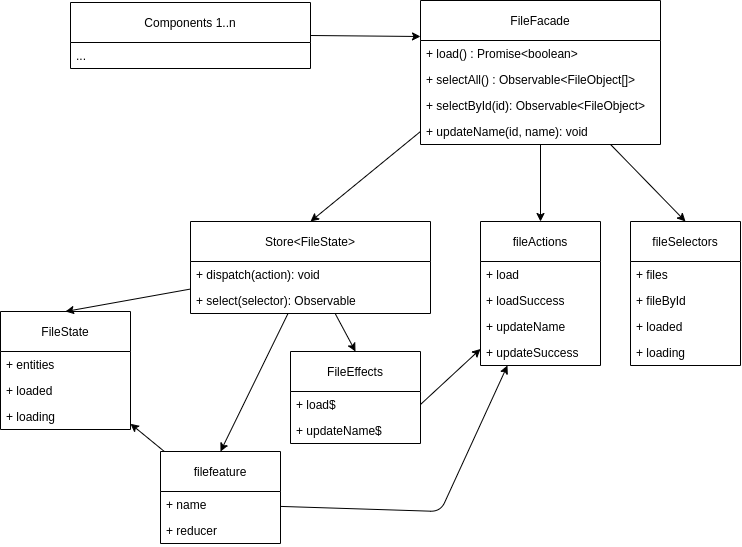
\includegraphics[height=10cm]{abbildungen/easy-state-comp.png}
\caption{FileStore Abhängigkeiten}
\label{fielStore-dependencies}
\end{figure}


\section{Datenstore mit WebSocket: herkömmlicher Ansatz}
\label{sec-datenstore-mit-websocket-herkoemmlicher-ansatz}

In diesem Abschnitt wird die Kombination der in \ref{sec-zentraler-redux-datenstore} und \ref{sec-sync-async-comm} beschriebenen Technologien betrachtet, insbesondere im Kontext von Datenänderungen. Der Prozess einer Datenänderung beginnt damit, dass der Client, der eine Änderung vornehmen möchte, eine entsprechende Action dispatched. Dies löst einen Side Effect aus, der wiederum einen Serveraufruf nach sich zieht. Auf dem Server wird der Änderungswunsch validiert und bei Erfolg umgesetzt. Bei erfolgreicher Änderung sendet der Server einen Statuscode zurück an den Client, der den Erfolg der Änderung bestätigt. Zudem ist es erforderlich, anderen Clients, die sich für Benachrichtigungen über Änderungen registriert haben, diese über eine WebSocket-Nachricht mitzuteilen. Die Clients reagieren nun auf den erhaltenen Statuscode oder die WebSocket-Benachrichtigung, indem sie eine Success-Action dispatchen. Die Success-Action aktiviert dann den Reducer, der wiederum den Store aktualisiert.


\begin{figure}[htbp]
\centering
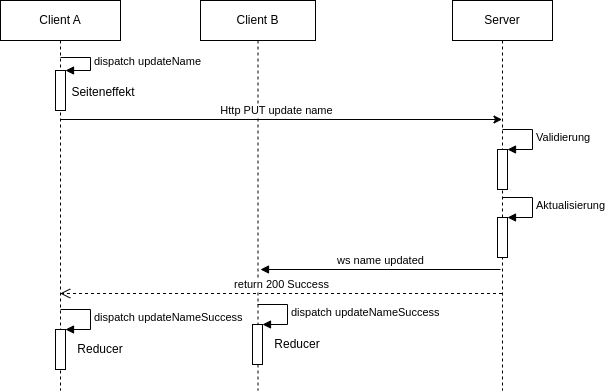
\includegraphics[height=10cm]{abbildungen/store-and-socket-herkoemmlich.png}
\caption{Interaktionsdiagramm: Datenstore mit WebSocket, herkömmlicher Ansatz}
\label{store-and-socket-herkoemmlich}
\end{figure}

Abbildung \ref{store-and-socket-herkoemmlich} illustriert diesen Ablauf anhand eines Interaktionsdiagramms. Es wird angenommen, dass Client A den Aktualisierungsvorgang initiiert, während Client B sich im Voraus für Aktualisierungsbenachrichtigungen angemeldet hat. Für die Implementierung jedes neuen Aktualisierungsvorgangs, der möglicherweise durch ein neues Feature entsteht, sind folgende Schritte erforderlich:

\begin{enumerate}
    \item Definition einer Action, die den Side Effect auslöst.
    \item Implementierung eines neuen HTTP-Endpunkts, sowohl server- als auch clientseitig.
    \item Implementierung des Side Effects.
    \item Implementierung der serverseitigen Validierungs- und Aktualisierungslogik.
    \item Implementierung eines neuen WebSocket-Endpunkts, ebenfalls server- und clientseitig.
    \item Definition einer Action, die die Reducer-Funktion auslöst.
    \item Implementierung der Reducer-Funktion zur Anpassung der Client-Daten.
\end{enumerate}

Die Notwendigkeit, diese Schritte für jede neue Funktionalität zu wiederholen, macht deutlich, dass dieser Ansatz langfristig sehr aufwendig ist. Um diese Herausforderungen zu bewältigen und den Implementierungsaufwand zu reduzieren, wurde \textit{YReduxSocket} entwickelt, das im nächsten Kapitel detailliert beschrieben wird.

%--------------YReduxSocket-------
%---------------------------------
\chapter{YReduxSocket}
\label{chap-y-redux-socket}

In diesem Kapitel widmen wir uns ausführlich dem Konzept des \textit{YReduxSocket}. Zunächst beginnen wir mit einer kompakten Einführung, in der wir das Konzept von \textit{YReduxSocket} kurz und prägnant umreißen. Anschließend entwickeln wir eine detaillierte generische Konzeption und Spezifikation, die sowohl einen Überblick als auch tiefergehende Einblicke in die Funktionsweise und Besonderheiten von \textit{YReduxSocket} bietet. Danach wird ein besonderer Fokus auf das Konsistenzverhalten von \textit{YReduxSocket} gelegt. Zum Abschluss des Kapitels erfolgt ein Vergleich zwischen dem \textit{YReduxSocket}-Ansatz und dem herkömmlichen Ansatz, wie er im Abschnitt \ref{sec-datenstore-mit-websocket-herkoemmlicher-ansatz} beschrieben wird. Dieser Vergleich soll die Vorzüge und möglichen Verbesserungen durch \textit{YReduxSocket} im Kontext bestehender Methoden hervorheben.

\section{Kurzbeschreibung}
\label{sec-kurzbeschreibung}

Die Kernidee von YReduxSocket zielt darauf ab, den in Abschnitt \ref{sec-datenstore-mit-websocket-herkoemmlicher-ansatz} dargestellten traditionellen Ansatz zu vereinfachen. Dies wird erreicht, indem Actions sowohl auf Server- als auch auf Clientseite definiert werden. Anstelle der Übermittlung der Action an den Store wird sie direkt an den Server gesendet. Der Server bedient sich eines einzigen HTTP-Endpunkts zum Empfangen der Action. Bei diesem Vorgang wird abhängig von der spezifischen Kennzeichnung der Action entschieden, welche Validierungen oder Datenbankmodifikationen erforderlich sind. Nach Abschluss der Operationen sendet der Server eine Action per WebSocket zurück an den Client. Diese Rückübermittlung erfolgt über eine bereits festgelegte Methode auf der Clientseite. Der Client muss in dieser Methode sicherstellen, dass die Action an den Store weitergeleitet wird, woraufhin der Reducer aktiv wird und entsprechende Anpassungen im Store vornimmt. Ein weiterer Vorteil dieses Ansatzes ist, dass bei Bedarf neuer Endpunkte auf zusätzliche Side Effects, die die Server-Client-Kommunikation betreffen, verzichtet werden kann. Um die Server-Client-Kommunikation mit YReduxSocket zu erweitern, sind folgende Schritte von einer Entwicklerin durchzuführen:
\begin{enumerate}
    \item Definition von zwei Actions auf der Client- und der Serverseite.
    \item Versenden einer Action vom Client an den Server über den bestehenden Endpunkt.
    \item Implementierung der Validierungs- und Anpassungslogik auf der Serverseite.
    \item Auslösen der serverseitigen Antwort über den bestehenden Client-Endpunkt unter Übergabe der zweiten Action.
    \item Implementierung der Reducer-Funktion auf der Clientseite zur Anpassung der Client-Daten.
\end{enumerate}

\begin{figure}[htbp]
\centering
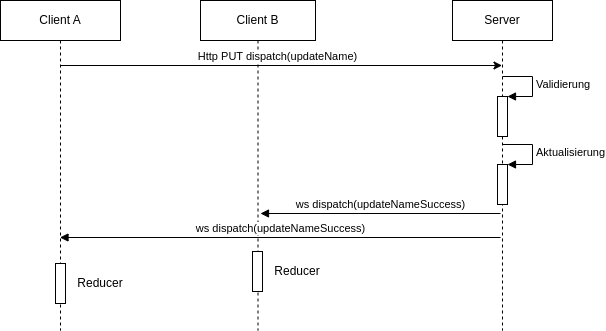
\includegraphics[height=8cm]{abbildungen/store-and-socket-y-redux.png}
\caption{Interaktionsdiagramm: Datenstore mit WebSocket, YReduxSocket}
\label{store-and-socket-y-redux-socket}
\end{figure}


Das Interaktionsdiagramm in Abbildung \ref{store-and-socket-y-redux-socket} illustriert die bei Datenänderungen involvierten Schritte. Ein Vergleich mit den Umsetzungsschritten bzw. mit dem Interaktionsdiagram (Abbildung \ref{store-and-socket-herkoemmlich}) in Abschnitt \ref{sec-datenstore-mit-websocket-herkoemmlicher-ansatz} zeigt, dass der YReduxSocket-Ansatz einen deutlich geringeren Implementierungsaufwand erfordert. Für einen detaillierten Vergleich sei auf Abschnitt \ref{sec-yr-vergleich-mit-herkoemmlichen-ansatz} verwiesen.

\section{Generische Konzeption und Spezifikation}
\label{sec-generische-konzeption-und-spezifikation}

Dieser Abschnitt konzentriert sich auf die generische Spezifikation von \textit{YReduxSocket}. Zuerst wird der initiale Verbindungsaufbau zwischen einem Client und dem Server dargelegt. Danach folgt eine Beschreibung des Anmeldeprozesses für Clients, um bei Datenänderungen entsprechend informiert zu werden. Weiterhin wird der HTTP-Endpunkt erläutert, der den Clients ermöglicht, Datenänderungen zu initiieren. Abschließend wird der WebSocket-Endpunkt vorgestellt, der von den Clients bereitgestellt wird, um vom Server über erfolgreiche Aktualisierungen benachrichtigt zu werden.

\subsection{Initialer Verbindungsaufbau}
\label{subsec-initialer-verbindungsaufbau}

Die Verwendung von \textit{YReduxSocket} erfordert zunächst das Aufbauen einer WebSocket-Verbindung zwischen dem Client und dem Server. Serverseitig muss dafür ein spezifischer Endpunkt bereitgestellt werden, den der Client ansprechen kann. Dieser initiiert die WebSocket-Verbindung. Clientseitig ist es erforderlich, beim ersten Laden des Skripts eine Verbindung zu diesem Endpunkt herzustellen. JavaScript stellt hierfür eine spezifische WebSocket-API (Application Programming Interface) zur Verfügung\footnote{\url{https://developer.mozilla.org/en-US/docs/Web/API/WebSockets\_API}}. Ähnlich bieten die meisten Server-Frameworks entsprechende Bibliotheken zur Nutzung von WebSockets an, wie zum Beispiel die WebSocket-Unterstützung in ASP.Net\footnote{\url{https://learn.microsoft.com/en-us/aspnet/core/fundamentals/websockets?view=aspnetcore-8.0}}.

Falls der Server eine Authentifizierung, beispielsweise mittels eines JsonWebTokens, verlangt, muss der Client sicherstellen, dass dieses Token sowohl beim Verbindungsaufbau als auch bei jeder nachfolgenden WebSocket-Nachricht mitgesendet wird. Auf der Serverseite ist es entscheidend, das übertragene Token bei jeder eingehenden Nachricht zu validieren.

Eine stabile Verbindung ist für den effektiven Einsatz von \textit{YReduxSocket} unerlässlich. Daher ist die Implementierung einer Fehlerbehandlung für Verbindungsschwierigkeiten von großer Bedeutung. Ein gängiger Ansatz ist das Anzeigen einer Fehlermeldung beim Nutzer während einer Unterbrechung der Verbindung, kombiniert mit dem Versuch, die Verbindung automatisch wiederherzustellen. Nach einer erfolgreichen Wiederverbindung ist es aus Gründen der Datenkonsistenz wichtig, alle Daten neu zu laden. Dies stellt sicher, dass keine Änderungen übersehen werden, die während einer Offline-Phase des Clients aufgetreten sein könnten.

Algorithmus \ref{alg-verbindungsaufbau-und-wiederherstellung-clientseitig} zeigt schematisch den Verbindungsaufbau und die Wiederherstellung. Zu Beginn wird eine WebSocket-Verbindung hergestellt und die Verbindungsinformationen in einer Variablen gespeichert. Es folgt eine Endlosschleife, in der in regelmäßigen Abständen, hier jede Sekunde, überprüft wird, ob die Verbindung noch besteht. Bei einer Unterbrechung wird dem Nutzer eine Fehlermeldung angezeigt und versucht, die Verbindung erneut aufzubauen. Nach erfolgreicher Wiederverbindung wird der \texttt{reduxState} auf den initialen Zustand zurückgesetzt, um ein erneutes Laden der Daten vom Server zu erzwingen.

\begin{algorithm}
\caption{Verbindungsaufbau und Wiederherstellung clientseitig}
\label{alg-verbindungsaufbau-und-wiederherstellung-clientseitig}
\begin{algorithmic}
    \State $\texttt{socketConnection} \gets \text{connect to server, store connection}$

    \While{$\text{true}$}
        \If{$\texttt{socketConnection} \text{ is not connected}$}
            \State \text{Display Reconnection message}
            \State $\texttt{socketConnection.reconnect()}$
            \If{$\texttt{socketConnection} \text{ is connected}$}
                \State $\texttt{reduxState} \gets \texttt{initialState}$ \Comment{Force a reload of data}
                \State \text{Remove Reconnecting message}
            \EndIf
        \EndIf
        \State \text{Wait for 1 second}
    \EndWhile
\end{algorithmic}
\end{algorithm}

\subsection{Anmeldung auf Datenänderungen}
\label{subsec-anmeldung-auf-datenaenderungen}

In einem typischen Szenario sind zahlreiche Clients gleichzeitig mit dem Server verbunden. Eine einfache Methode, Datenänderungen über den WebSocket zu verteilen, wäre die Verwendung eines Broadcasts, bei dem die Aktualisierungsnachrichten an alle verbundenen Clients gesendet werden. Dieser Ansatz führt jedoch zu einer Flut unnötiger Nachrichten, was die Skalierbarkeit des Systems beeinträchtigen kann.

Ein effizienterer Ansatz besteht darin, die Clients in spezifische Gruppen zu organisieren. Hierbei registrieren sich die Clients für Updates zu Datenänderungen, die für sie relevant sind. Diese Vorgehensweise ermöglicht eine gezielte Nachrichtenverteilung und reduziert die Netzwerklast. Die Gruppeneinteilung bei "`Yoshie.io"' ist in Abbildung \ref{abb-ws-groups} dargestellt. Nachfolgend wird ein detaillierter Blick auf diese Gruppenstruktur und ihre Funktionsweise geworfen.

\begin{figure}[htbp]
\centering
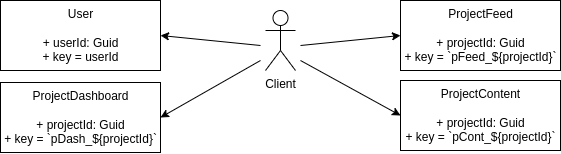
\includegraphics[height=4cm]{abbildungen/ws-groups.png}
\caption{WebSocket-Gruppen bei "`Yoshie.io"'}
\label{abb-ws-groups}
\end{figure}


In "`Yoshie.io"' sind Datensätze als sogenannte \texttt{YNode} in Projekten strukturiert. Ein Projekt ist dabei selbst eine \texttt{YNode}. Jeder Datensatz verfügt über eine \texttt{projectId}, die auf ein bestimmtes Projekt verweist. Für die eindeutige Identifikation einer Gruppe wird ein spezieller Schlüssel definiert, der für die jeweilige Gruppe einzigartig ist. Bei den in Abbildung \ref{abb-ws-groups} dargestellten Gruppen wird dies durch Verwendung der einzigartigen ID der betreffenden Entität – in diesem Fall der Nutzer oder Projekte – erreicht. Existieren mehrere Gruppen derselben Entitätsart (hier Projekte), wird ein Präfix hinzugefügt, um Eindeutigkeit zu gewährleisten.

Stellt ein Client eine Verbindung zum WebSocket her, wird er automatisch der Gruppe \texttt{User} zugeordnet. Die Information über die UserId des Clients wird im Authentifizierungstoken übermittelt. Bei einem Verbindungsabbruch wird der Client wieder aus der Gruppe \texttt{User} entfernt. Diese Gruppe dient dazu, WebSocket-Nachrichten an alle Clients zu senden, die mit demselben Benutzerkonto verbunden sind. Ein praktisches Beispiel hierfür ist die Erstellung eines neuen Projekts. Zum Zeitpunkt der Erstellung ist kein anderer Nutzer außer dem Ersteller mit dem Projekt verbunden, sodass nur diesem Nutzer die Information übermittelt werden muss. Auf diese Weise kann sichergestellt werden, dass der Nutzer, wenn er sowohl über sein Smartphone als auch über seinen Desktop verbunden ist, das neu angelegte Projekt sofort auf beiden Geräten sieht.

Der Client hat die Option, alle Projekte, zu denen er Zugang hat, zu laden. Sobald dies geschieht, werden die Projektdaten in seinem Redux-basierten Speicher (Store) abgelegt. Um Live-Updates zu Änderungen dieser Projekte zu erhalten – beispielsweise Modifikationen einzelner Datenwerte wie Namen – ist es notwendig, dass der Client sich für die Gruppe \texttt{ProjektDashboard} registriert. Dies betrifft alle \texttt{projectIds}, die geladen wurden. Durch diese Registrierung ist der Client in der Lage, Echtzeit-Updates zu erhalten, sobald Änderungen an den Projektdaten vorgenommen werden.

Ein Client kann auch ein einzelnes Projekt öffnen, was bedeutet, dass alle Inhalte dieses Projekts in den Store geladen werden. Unter Projektinhalt versteht man bei "`Yoshie.io"' \texttt{YNode}-Entitäten, denen die \texttt{projectId} des jeweiligen Projekts zugeordnet ist. Beispiele hierfür sind Dateien, Tags oder Aufgaben. Ein Client kann jeweils nur Inhalte eines Projekts geladen haben. Beim Laden eines Projekts muss sich der Client für die Gruppe \texttt{ProjectContent} der entsprechenden \texttt{projectId} registrieren. Hatte er zuvor Inhalte eines anderen Projekts geladen, muss er sich von dieser Gruppe abmelden.

Schließlich gibt es die Gruppe \texttt{ProjectFeed}. Ein Projekt-Feed entspricht Einträgen welche Aktualisierungen eines Projekts bzw. dessen Inhalte beschreiben. Jedes Projekt bietet eine eigene Ansicht des Feed. Zudem gibt es eine Gesamtübersicht, der den Feed aller Projekte eines Nutzers zusammenfasst. Lädt der Client einen spezifischen Projekt-Feed in seinen Store, muss er sich für die Gruppe des entsprechenden Projekts registrieren und sich gegebenenfalls vom vorherigen Projekt-Feed abmelden. Beim Laden der Gesamtübersicht erfolgt eine Anmeldung bei allen  \texttt{ProjectFeed}-Gruppen, zu denen der Client Zugriff hat, ähnlich der Registrierung bei der \texttt{ProjectDashboard}-Gruppe.

\subsection{Definition von Actions}
\label{subsec-definition-von-actions}

Wie bereits in Abschnitt \ref{subsec-actions} erläutert, können Actions mit der \texttt{dispatch}-Methode an den Store übermittelt werden. Diese Actions dienen entweder dazu, eine Reducer-Funktion aufzurufen oder einen Side Effect auszulösen. Mit der Einführung von \textit{YReduxSocket} ergibt sich jedoch eine leichte Modifikation dieses Prozesses. Es ist wichtig, zwischen zwei Arten von Actions zu unterscheiden: solchen, die vom Client an den Server gesendet werden, um beispielsweise eine Datenänderung zu veranlassen (siehe Abschnitt \ref{subsec-http-endpunkt-dispatch-action}), und solchen, die den Erfolg einer Operation vom Server an den Client übermitteln (siehe Abschnitt \ref{subsec-web-socket-endpunkt-disptach-success-action}).

Zur klaren Unterscheidung dieser beiden Action-Typen werden die Begriffe \textit{trigger-Action} und \textit{success-Action} eingeführt. Eine \textit{trigger-Action} bezieht sich auf eine Action, die vom Client an den Server gesendet wird, während eine \textit{success-Action} eine Action ist, die vom Server zum Client gesendet wird, um den erfolgreichen Abschluss einer Operation zu signalisieren.

Bei der Verwendung von \textit{YReduxSocket} ist es erforderlich, Actions sowohl auf der Client- als auch auf der Serverseite zu definieren. Auf der Clientseite bleibt die Definition der Actions gemäß Abschnitt \ref{subsec-actions} unverändert. Allerdings entfallen die herkömmlichen HTTP-Aufrufe als Side Effects, da \textit{trigger-Actions} nun direkt an den Server gesendet werden. Die \textit{success-Actions} lösen weiterhin den Aufruf einer Reducer-Funktion aus.

\begin{figure}[htbp]
\centering
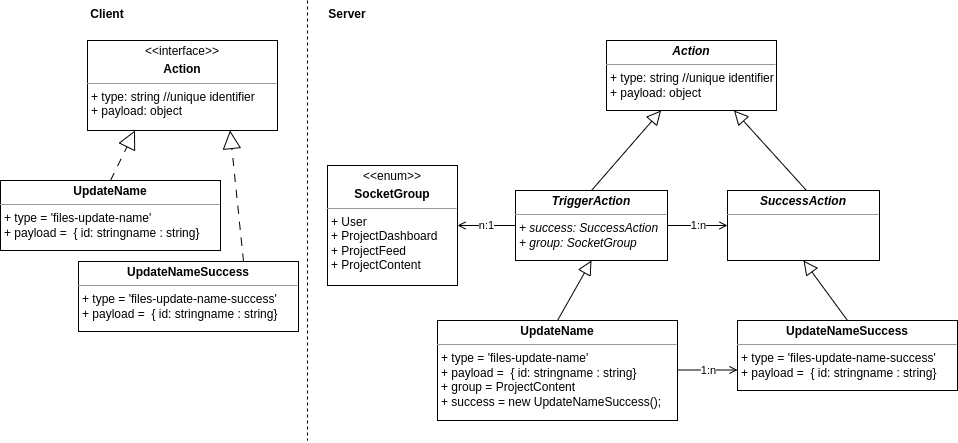
\includegraphics[height=7.5cm]{abbildungen/y-redux-socket-actions.png}
\caption{Klassendiagramm: YReduxSocket Actions}
\label{abb-klassendiagramm-y-redux-socket-actions}
\end{figure}

Auf der Serverseite ist nun ebenfalls eine Definition der Actions erforderlich. Hierbei muss für jede Action eine eindeutige Identifikation sowie der zu übermittelnde Payload festgelegt werden. Zusätzlich muss bei \textit{trigger-Actions} spezifiziert werden, welche \textit{success-Actions} im Falle einer erfolgreichen Operation auf welcher WebSocket-Gruppe (siehe Abschnitt \ref{subsec-anmeldung-auf-datenaenderungen}) zurückgemeldet werden sollen. Abbildung \ref{abb-klassendiagramm-y-redux-socket-actions} veranschaulicht das beschriebene nochmals als Klassendiagramm. Dabei handelt es sich bei \texttt{TriggerAction} und bei \texttt{SuccessAction} um abstrakte Basisklassen, die Actions \texttt{UpdateName} und \texttt{UpdateNameSuccess} sind Beispielimplementierungen dieser Basisklassen. In der Regel existieren mehrere solcher Implementierungen.

\subsection{HTTP-Endpunkt \texttt{dispatch(triggerAction)}}
\label{subsec-http-endpunkt-dispatch-action}

\textit{YReduxSocket} setzt voraus, dass der Server einen HTTP-Endpunkt bereitstellt, der es dem Client ermöglicht, \texttt{triggerActions} direkt an den Server zu senden. Dies unterscheidet sich vom konventionellen Ansatz, bei dem das Auslösen einer Aktion Side Effects erzeugt, die wiederum spezifische HTTP-Endpunkte aufrufen.

\begin{figure}[htbp]
\centering
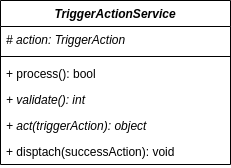
\includegraphics[height=3.5cm]{abbildungen/trigger-action-service.png}
\caption{UML-Klassendiagramm des \texttt{TriggerActionService}}
\label{abb-klassendiagramm-triggeractionservice}
\end{figure}

Die abstrakte Klasse \texttt{TriggerActionService} auf dem Server, dargestellt im UML-Klassendiagramm in Abbildung \ref{abb-klassendiagramm-triggeractionservice}, ist zentral für dieses Konzept. Für jede \texttt{TriggerAction} sollte eine entsprechende Implementierung dieses Services existieren. In dieser Implementierung sind die abstrakten Methoden \texttt{validate()} und \texttt{act(triggerAction): object} zu definieren. Die Methode \texttt{validate()} analysiert den Payload der \texttt{TriggerAction} und gibt einen HTTP-Statuscode zurück, wobei der Code 200 (OK) eine erfolgreiche Validierung anzeigt. Die Methode \texttt{act} führt die notwendige Aktualisierung durch und liefert ein Objekt als Payload für die an den Client zu sendende \texttt{SuccessAction}.

Bei Eintreffen einer \texttt{TriggerAction} über den \texttt{dispatch}-Endpunkt auf dem Server wird die Methode \texttt{process(): boolean} der zugehörigen \texttt{TriggerActionService}-Implementierung aufgerufen. Algorithmus \ref{alg-process-trigger-action-service} veranschaulicht den Ablauf dieser Methode. Zunächst erfolgt eine Validierung der Anfrage. Bei einem Fehler wird der entsprechende HTTP-Statuscode zurückgegeben. Bei erfolgreicher Validierung wird die Aktualisierung durchgeführt, der Payload für die \texttt{SuccessAction} festgelegt und diese mittels WebSocket an alle Clients in der entsprechenden Gruppe versendet. Dieser Prozess ist in einem Try-Catch-Block eingebettet, um bei auftretenden Fehlern einen internen Serverfehler an den Client melden zu können.

\begin{algorithm}
\caption{Methode \texttt{process()} in der Klasse \texttt{TriggerActionService}}
\label{alg-process-trigger-action-service}
\begin{lstlisting}
public process() {
    var status = validate();
    if(status != 200) {
        logError(status);
        return StatusCode(status);
    }
    
    try {
        var payload = act(this.action);
        this.action.success.payload = payload;
        dispatch(this.action.group, this.action.success);
        return Ok(payload);
    } catch(e) {
        logError(e);
        return InternalServerError();
    }
}
\end{lstlisting}
\end{algorithm}

\subsection{WebSocket Endpunkt \texttt{dispatch(successAction)}}
\label{subsec-web-socket-endpunkt-disptach-success-action}

Wie im vorherigen Abschnitt erläutert, benachrichtigt der Server Clients, die sich für eine durch eine \texttt{TriggerAction} definierte Gruppe registriert haben, mittels eines WebSocket-Aufrufs. Dieser Aufruf erfolgt über eine von den Clients bereitgestellte WebSocket-Methode, wobei die entsprechende \texttt{SuccessAction} (welche durch die \texttt{TriggerAction} definiert wurde) übergeben wird. 

Auf der Clientseite wird in dieser Methode einfach die \texttt{dispatch}-Funktion des Redux-basierten Stores aufgerufen. Dies führt in der Regel dazu, dass eine Reducer-Funktion aktiviert wird, welche den Store entsprechend der erhaltenen \texttt{SuccessAction} aktualisiert. Es ist wichtig zu beachten, dass die Reducer-Funktion zusätzlich zur \texttt{SuccessAction} auf der Clientseite implementiert werden muss.

\section{Analyse des Konsistenzverhaltens von YReduxSocket}
\label{sec-konsistenzverhalten}

Dieser Abschnitt konzentriert sich auf eine detaillierte Analyse des Konsistenzverhaltens von \textit{YReduxSocket}. Zunächst wird vorgestellt wie in \texttt{YReduxSocket} Transaktionen eingesetzt werden um die ACID Eigenschaften zu erreichen. Danach, werden verschiedene Konsistenzmodelle, die auf der Clientseite anwendbar sind, schrittweise vorgestellt und untersucht. Ziel ist es, zu evaluieren, inwiefern \textit{YReduxSocket} diesen Modellen entspricht oder Anpassungen erfordert.

\subsection{Transaktionen}
\label{subsec-transactions-yredux-socket}

Wie bereits in Abschnitt \ref{sec-acid-prinzipien} erläutert, setzt der Einsatz von \textit{YReduxSocket} eine Datenbank voraus, die Transaktionen mit ACID-Eigenschaften unterstützt.

Algorithmus \ref{alg-process-trigger-action-service} beschreibt die Verarbeitung von \texttt{TriggerActions} durch den Server. Während dieser Verarbeitung ist es entscheidend, dass der Aufruf der \texttt{act()}-Methode, welche die Datenbankmodifikationen durchführt, innerhalb einer Transaktion stattfindet. Dies gewährleistet, dass bei einer \texttt{SuccessAction} davon ausgegangen werden kann, dass die Änderungen atomar, konsistent, isoliert und dauerhaft erfolgt sind (siehe Abschnitt \ref{sec-acid-prinzipien}).

Um die Notwendigkeit der Transaktionsverarbeitung in jeder Implementierung der abstrakten Basisklasse \texttt{TriggerActionService} zu vermeiden, wird eine neue Methode \texttt{actBase(triggerAction): object} im \texttt{TriggerActionService} eingeführt. Diese Methode wird im Algorithmus \ref{alg-process-trigger-action-service} anstelle der \texttt{act()}-Methode aufgerufen. Algorithmus \ref{alg-transaction-relational-database} aus Abschnitt \ref{sec-acid-prinzipien} illustriert eine mögliche Implementierung dieser Methode.


\subsection{Monotones Lesen}
\label{subsec-monotones-lesen}

Tanenbaum und van Steen definieren das clientbasierte Konsistenzmodell für monotone Lesevorgänge wie folgt:

\begin{quote}
"`Wenn ein Prozess den Wert eines Datenelments $x$ liest, gibt jede anschließende Leseoperation dieses Prozesses auf $x$ stets denselben oder einen aktuelleren Wert zurück."' \cite[322]{tanenbaum_verteilte_2008}
\end{quote}

Wie bereits erwähnt, stützt sich \textit{YReduxSocket} auf die Verwendung einer einzigen Datenbank, die als zentrale Wahrheitsquelle (Single Source of Truth) angesehen wird. Diese Datenbank wird ausschließlich durch Aktionen modifiziert, die innerhalb von Transaktionen stattfinden und die ACID-Prinzipien einhalten.

Eine Leseoperation in \textit{YReduxSocket} wird durch eine \texttt{TriggerAction} und eine \texttt{SuccessAction} umgesetzt. Möchte ein Client eine Leseoperation initiieren, sendet er eine \texttt{TriggerAction} an den Server (z.B. \texttt{loadFile(id)}). Der Server liest daraufhin den Datensatz aus der Datenbank und sendet ihn mit einer \texttt{SuccessAction} (z.B. \texttt{loadFileSuccess(file)}) an den anfragenden Client zurück. Die gelesenen Daten werden für den Client sichtbar, sobald er die \texttt{SuccessAction} erhält.

Die eingesetzten Transaktionen bei Schreibvorgängen gewährleisten, dass nur konsistente Datenwerte nach außen hin sichtbar werden. Dies entspricht der Konsistenzeigenschaft der ACID-Prinzipien, welche sicherstellt, dass inkonsistente Zwischenergebnisse während der Transaktionen verborgen bleiben. Somit sind die von einem Client gelesenen Werte stets konsistent. Zusätzlich sorgt die Dauerhaftigkeitseigenschaft der ACID-Prinzipien dafür, dass einmal geschriebene Daten beständig und zuverlässig gespeichert werden. 

Wenn ein Client denselben Datensatz zu verschiedenen Zeitpunkten liest, garantieren die ACID-Prinzipien, dass immer konsistente und bestätigte Daten übermittelt werden. Der Client erhält zwei \texttt{SuccessActions}, wobei die zuletzt eintreffende die vorherige aktualisiert. Jedoch kann nicht garantiert werden, dass diese \texttt{SuccessAction} stets die aktuellere ist, da sich die Aktionen auf dem Weg vom Server zum Client überholen können. Das Konsistenzmodell des monotonen Lesens kann daher nicht vollständig sichergestellt werden. In den meisten Anwendungsfällen ist dies jedoch nicht erforderlich. Ändert ein Teilnehmer im System den gelesenen Datensatz, wird an alle Clients, die diese Daten gelesen hatten, eine aktualisierende \texttt{SuccessAction} gesendet, wodurch der Datensatz auf den neuesten Stand gebracht wird. Dieses Verhalten wird als "`eventual consistency"' bezeichnet, was bedeutet, dass der Zustand des Clients über die Zeit mit dem Zustand in der Datenbank konvergiert \cite[319-321]{tanenbaum_verteilte_2008}.

\subsection{Monotones Schreiben}
\label{subsec-monotones-schreiben}

Zunächst die Definition des Konsistenzmodells laut Tannenbaum und van Steen:

\begin{quote}
"`Eine Schreiboperation eines Prozesses an einem Datenelement $x$ wird abgeschlossen, bevor eine folgende Schreiboperation auf $x$ durch denselben Prozess erfolgen kann."' \cite[323]{tanenbaum_verteilte_2008}
\end{quote}

\textit{YReduxSocket} kann das Prinzip des monotonen Schreibens nicht vollständig umsetzen. Wenn ein Client kurz hintereinander zwei \texttt{TriggerActions} sendet, die denselben Datensatz ändern sollen, ist die Reihenfolge der Ausführung nicht garantiert. Die zuerst ankommende Aktion wird angewendet, gefolgt von der nachfolgenden. Auch hier werden zwei \texttt{SuccessActions} versendet, wobei die zuletzt beim Client eintreffende Aktion den Store abschließend aktualisiert. Dieses Konsistenzverhalten ist für viele Anwendungsfälle ausreichend. Für Szenarien, die eine stärkere Konsistenz erfordern, kann \textit{YReduxSocket} durch die Implementierung eines speziellen Algorithmus erweitert werden, wodurch die Konsistenzmodelle des monotonen Lesens und Schreibens erfüllt werden. Weitere Details dazu finden sich in Abschnitt \ref{subsec-algorithmus von haverbeke}.

\subsection{Read Your Writes}
\label{subsec-read-your-writes}

Dieser Abschnitt stützt sich ebenfalls auf eine Definition von Tanenbaum und van Steen:

\begin{quote}
"`Die Folge einer Schreiboperation eines Prozesses auf das Datenelement $x$ wird für eine anschließende Leseoperation auf $x$ durch denselben Prozess stets sichtbar sein."' \cite[324]{tanenbaum_verteilte_2008}
\end{quote}

Dank der bei Schreibvorgängen eingesetzten Transaktionen kann die ACID-Eigenschaft der Dauerhaftigkeit die Sichtbarkeit der Schreiboperationen für nachfolgende Leseoperationen garantieren. Wenn ein Client eine TriggerAction sendet, die eine Modifikation eines Datensatzes auslösen soll, wird diese Modifikation bei erfolgreicher Validierung innerhalb einer Transaktion durchgeführt. Ist der Vorgang erfolgreich, bleibt die Änderung dauerhaft in der Datenbank gespeichert. Jeder nachfolgende Lesevorgang, der auf diesen Datensatz zugreift, liefert als Ergebnis einen Wert, der auf dieser Transaktion basiert – entweder diesen Wert oder einen aktuelleren.

\subsection{Write Follows Reads}
\label{subsec-write-follows-reads}

Das abschließend untersuchte Konsistenzmodell basiert auch auf einer Definition von Tanenbaum und van Steen:

\begin{quote}
"`Einer Schreiboperation eines Prozesses auf ein Datenelement $x$, die auf eine vorherige Leseoperation auf $x$ durch denselben Prozess folgt, wird garantiert, dass sie auf demselben oder einem aktuelleren Wert von $x$ stattfindet."' \cite[326]{tanenbaum_verteilte_2008}
\end{quote}

Auch diese Eigenschaft wird auch von \textit{YReduxSocket} erfüllt. Wenn ein Wert aus der Datenbank gelesen wird, wird dieser mittels einem dispatchen einer \texttt{SuccessAction} in den Client-Store geladen. Schreiboperationen basieren nun auf diesem Wert. Der Client sendet also einen modifizierten Wert an den Server, der auf dem zuvor geladenen Wert basiert. Auch hier unterstützt die Dauerhaftigkeitseigenschaft der ACID-Prinzipien die Konsistenz, da der Wert direkt aus der Datenbank geladen wurde. Daher kann zum Zeitpunkt des Eintreffens der TriggerAction, die eine Änderung auslösen soll, nur dieser Wert oder ein aktuellerer in der Datenbank vorhanden sein.

\subsection{Algorithmus von Haverbeke}
\label{subsec-algorithmus von haverbeke}

Wie in vorangegangenen Abschnitten erörtert, unterstützt \textit{YReduxSocket} die clientseitigen Konsistenzmodelle \textit{Read Your Writes} und \textit{Write Follows Read}. Die Einhaltung der Modelle \textit{Monotones Lesen} und \textit{Monotones Schreiben} kann jedoch nicht vollständig gewährleistet werden. Für Einsatzszenarien, die eine strikte Konsistenz verlangen, erweist sich das bisher vorgestellte Konzept als nicht voll ausreichend. Diese Problematik wurde bei der Entwicklung des integrierten Editors der Plattform "`yoshie.io"' offensichtlich, welcher eine nahtlose kollaborative Bearbeitung durch mehrere Nutzer ermöglichen soll.

Zur Gewährleistung einer strengen Konsistenz wurde \textit{YReduxSocket} um den Haverbeke-Algorithmus erweitert. Diese Erweiterung basiert wesentlich auf einem Blogbeitrag von Marijn Haverbeke \cite{haverbeke_collaborative_2015}. Die folgenden Ausführungen stützen sich ebenfalls auf diesen Beitrag sowie auf einen Entwicklerleitfaden\footnote{\url{https://prosemirror.net/docs/guide/\#collab}}, der die Umsetzung kollaborativen Editierens mittels des Open-Source-Frameworks Prosemirror beschreibt. Prosemirror besteht aus einer Reihe von JavaScript-Bibliotheken, die für die Entwicklung kollaborativer Editoren verwendet werden können und hauptsächlich von Marijn Haverbeke entwickelt wurden.

%TODO noch nicht fertig
Der Algorithmus besteht aus zwei Teilen. Ein Teil muss am Server eingebaut und ein Teil am Client. Dabei wird auf sogenannten \texttt{Steps} aufgebaut. Ein \texttt{Step} besteht dabei aus aus einer \texttt{SuccessAction} und einer fortlaufenden Versionsnummer.


\begin{algorithm}
\caption{Serverseite des Haverbeke-Algorithmus}
\label{alg-hverbeke-server}
\begin{lstlisting}
//action erweitern um clientId und version

private triggerActions = [];

processHaverbeke() {
    //Falls die Versionsnummern nicht übereinstimmen wird nichts unternommen
    if(this.action.version != this.triggerActions.length) return;

    var status = validate();
    if(status != 200) {
        logError(status);
        return StatusCode(status);
    }

    var pushed = false;
    try {
        var payload = act(this.action);
        this.action.success.payload = payload
        
        //Action wurde auf Datenspeicher angewandt
        triggerActions.push(this.action);
        pushed = true;

        dispatch(this.action.group, this.action.success);
        return Ok(payload);
    } catch(e) {
        if(pushed) this.triggerActions.pop();
        
        logError(e);
        return InternalServerError();
    }
}

print("Hallo Welt");
\end{lstlisting}
\end{algorithm}


\begin{algorithm}
\caption{Clientseite des Haverbeke-Algorithmus}
\label{alg-hverbeke-client}
\begin{lstlisting}
print("Hallo Welt");
\end{lstlisting}
\end{algorithm}

\section{Vergleich mit herkömmlichen Ansatz}
\label{sec-yr-vergleich-mit-herkoemmlichen-ansatz}

%--------------Implementierung und Tests-------
%----------------------------------------------
\chapter{Implementierung und Tests}
\label{chap-implementierung-und-tests}

\section{Software Architektur}
\label{sec-impl-architektur}

\section{Client: Angular}
\label{sec-impl-angular}

\section{Server: ASP.Net}
\label{sec-impl-asp-net}

\section{Vergleich mit herkömmlichen Ansatz}
\label{sec-impl-vergleich-mit-herkoemmlichen-ansatz}

%--------------Fazit-------
%--------------------------
\chapter{Fazit}
\label{chap-fazit}

\section{Zusammenfassung}
\label{sec-fazit-zusammenfassung}

\section{Verbesserungspotential}
\label{sec-fazit-verbesserungsprotential}

\printbibliography

\end{document}
